\documentclass[tikz,border=7pt]{standalone}
\usepackage[T1]{fontenc}
\usepackage{helvet}
\usepackage{amsmath,amssymb}
\renewcommand{\familydefault}{\sfdefault}
\usetikzlibrary{arrows.meta,positioning,fit,calc,backgrounds}

\definecolor{navy}{HTML}{17324D}
\definecolor{blue}{HTML}{2F6B9A}
\definecolor{cyan}{HTML}{DCEFF5}
\definecolor{teal}{HTML}{278C82}
\definecolor{green}{HTML}{DFF2E7}
\definecolor{orange}{HTML}{E58B3A}
\definecolor{gold}{HTML}{F8E6B6}
\definecolor{purple}{HTML}{7457A6}
\definecolor{lavender}{HTML}{E9E2F5}
\definecolor{red}{HTML}{C95555}
\definecolor{rose}{HTML}{F8E1E1}
\definecolor{ink}{HTML}{263442}
\definecolor{muted}{HTML}{607385}
\definecolor{panel}{HTML}{F6F8FA}

\begin{document}
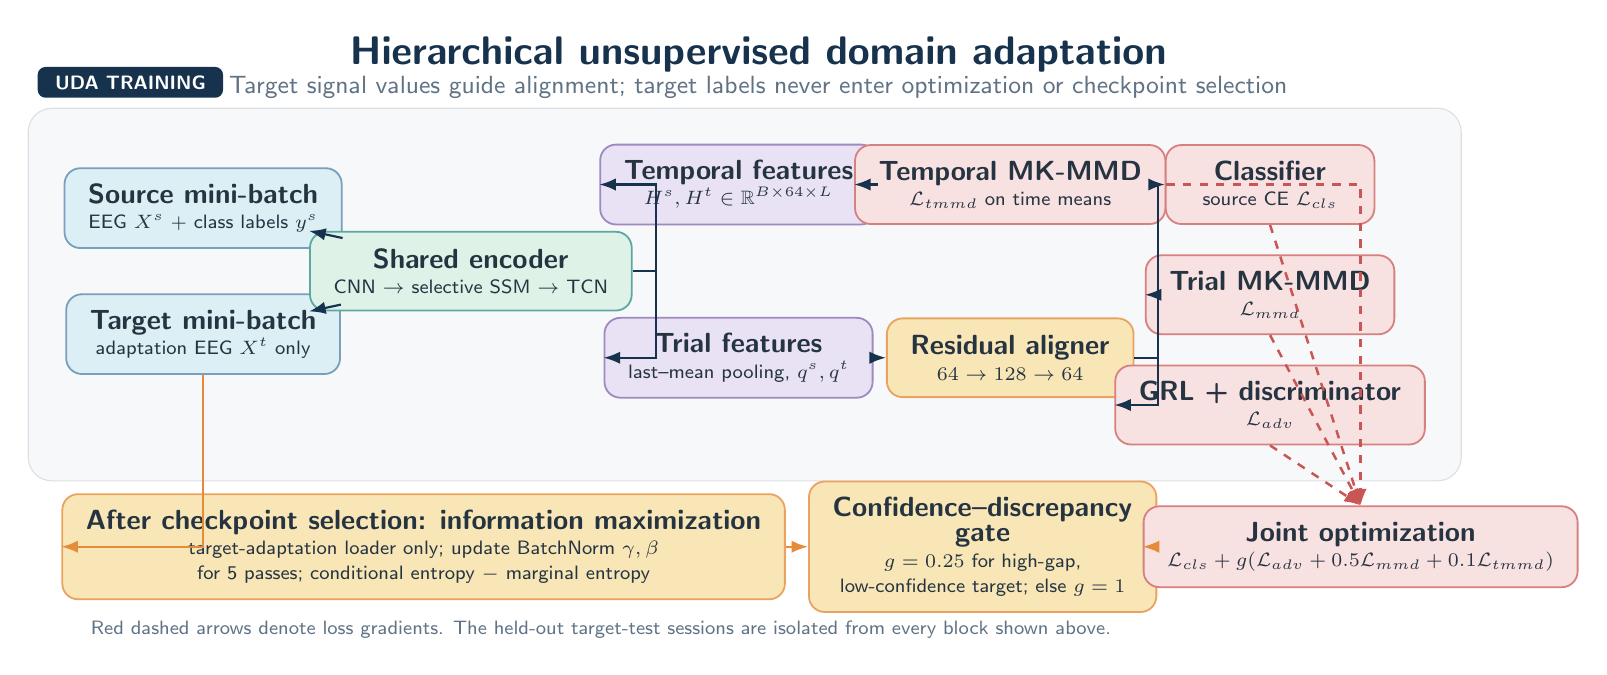
\begin{tikzpicture}[
  font=\sffamily,
  >=Latex,
  flow/.style={-{Latex[length=2.1mm]}, line width=0.78pt, draw=navy},
  grad/.style={-{Latex[length=2.1mm]}, line width=0.9pt, draw=red, dashed},
  card/.style={rounded corners=2mm, minimum height=10mm, align=center,
               draw=navy!35, line width=0.65pt, fill=white, text=ink,
               inner xsep=3mm, inner ysep=2mm},
  data/.style={card, fill=cyan, draw=blue!65},
  feature/.style={card, fill=green, draw=teal!75},
  adapt/.style={card, fill=gold, draw=orange!80},
  loss/.style={card, fill=rose, draw=red!75},
  state/.style={card, fill=lavender, draw=purple!70},
  tag/.style={font=\bfseries\scriptsize, text=white, rounded corners=1mm,
              inner xsep=2.2mm, inner ysep=1.1mm},
  note/.style={font=\scriptsize, text=muted, align=center}
]

\node[font=\bfseries\Large, text=navy] at (8.8,7.20)
  {Hierarchical unsupervised domain adaptation};
\node[font=\small, text=muted] at (8.8,6.78)
  {Target signal values guide alignment; target labels never enter optimization or checkpoint selection};

\node[data, minimum width=3.1cm] (src) at (1.75,5.25)
  {\textbf{Source mini-batch}\\[-1mm]\scriptsize EEG $X^s$ + class labels $y^s$};
\node[data, minimum width=3.1cm] (tgt) at (1.75,3.65)
  {\textbf{Target mini-batch}\\[-1mm]\scriptsize adaptation EEG $X^t$ only};
\node[feature, minimum width=3.3cm] (enc) at (5.15,4.45)
  {\textbf{Shared encoder}\\[-1mm]\scriptsize CNN $\rightarrow$ selective SSM $\rightarrow$ TCN};
\draw[flow] (src) -- (enc.north west);
\draw[flow] (tgt) -- (enc.south west);

\node[state, minimum width=3.05cm] (temporal) at (8.55,5.55)
  {\textbf{Temporal features}\\[-1mm]\scriptsize $H^s,H^t\in\mathbb{R}^{B\times64\times L}$};
\node[state, minimum width=3.05cm] (pooled) at (8.55,3.35)
  {\textbf{Trial features}\\[-1mm]\scriptsize last--mean pooling, $q^s,q^t$};
\draw[flow] (enc.east) -- ++(0.3,0) |- (temporal.west);
\draw[flow] (enc.east) -- ++(0.3,0) |- (pooled.west);

\node[loss, minimum width=2.75cm] (tmmd) at (12.0,5.55)
  {\textbf{Temporal MK-MMD}\\[-1mm]\scriptsize $\mathcal{L}_{tmmd}$ on time means};
\node[adapt, minimum width=2.75cm] (aligner) at (12.0,3.35)
  {\textbf{Residual aligner}\\[-1mm]\scriptsize $64\rightarrow128\rightarrow64$};
\draw[flow] (temporal) -- (tmmd);
\draw[flow] (pooled) -- (aligner);

\node[loss, minimum width=2.65cm] (ce) at (15.30,5.55)
  {\textbf{Classifier}\\[-1mm]\scriptsize source CE $\mathcal{L}_{cls}$};
\node[loss, minimum width=2.65cm] (mmd) at (15.30,4.15)
  {\textbf{Trial MK-MMD}\\[-1mm]\scriptsize $\mathcal{L}_{mmd}$};
\node[loss, minimum width=2.65cm] (adv) at (15.30,2.75)
  {\textbf{GRL + discriminator}\\[-1mm]\scriptsize $\mathcal{L}_{adv}$};
\draw[flow] (aligner.east) -- ++(0.30,0) |- (ce.west);
\draw[flow] (aligner.east) -- ++(0.30,0) |- (mmd.west);
\draw[flow] (aligner.east) -- ++(0.30,0) |- (adv.west);

\node[adapt, minimum width=3.30cm] (gate) at (11.65,0.95)
  {\textbf{Confidence--discrepancy}\\[-1mm]\textbf{gate}\\[-1mm]\scriptsize $g=0.25$ for high-gap,\\[-1mm]\scriptsize low-confidence target; else $g=1$};
\node[loss, minimum width=4.15cm] (total) at (16.45,0.95)
  {\textbf{Joint optimization}\\[-1mm]\scriptsize $\mathcal{L}_{cls}+g(\mathcal{L}_{adv}+0.5\mathcal{L}_{mmd}+0.1\mathcal{L}_{tmmd})$};
\draw[flow, draw=orange] (tgt.south) |- (gate.west);
\draw[grad] (tmmd.east) -| (total.north);
\draw[grad] (ce.south) -- (total.north);
\draw[grad] (mmd.south) -- (total.north);
\draw[grad] (adv.south) -- (total.north);
\draw[flow, draw=orange] (gate) -- (total);

\node[adapt, minimum width=5.9cm] (im) at (4.55,0.95)
  {\textbf{After checkpoint selection: information maximization}\\[-1mm]
   \scriptsize target-adaptation loader only; update BatchNorm $\gamma,\beta$\\[-1mm]
   \scriptsize for 5 passes; conditional entropy $-$ marginal entropy};
\draw[flow, draw=orange] (tgt.south) |- (im.west);

\begin{scope}[on background layer]
  \node[rounded corners=3mm, fill=panel, draw=navy!15,
        fit=(src)(tgt)(enc)(temporal)(pooled)(tmmd)(aligner)(ce)(mmd)(adv),
        inner sep=4.5mm] (training) {};
\end{scope}
\node[tag, fill=navy, anchor=south west] at ($(training.north west)+(0.12,0.12)$)
  {UDA TRAINING};
\node[note, anchor=west] at (0.20,-0.10)
  {Red dashed arrows denote loss gradients. The held-out target-test sessions are isolated from every block shown above.};

\end{tikzpicture}
\end{document}
